\section{A PROGRAMAÇÃO GENÉTICA}\label{sec:1pg-apg}

Um breve sumário da programação genética foi incluído na Introdução. Entretanto, é preciso aprofundar os conceitos mencionados. Neste capítulo são abordados os aspectos mais específicos da representação da Figura ~\ref{fig:intro-repgp}, isto é, o que exatamente são os caracteres $abcdef$ em cada problema. Uma visão geral do ciclo evolutivo artificial é incluída neste capítulo, e servirá de base para os próximos, já que o objetivo é implementar o algoritmo completo.

A aprendizagem evolucionária, em geral, pode ser sumarizada com etapas semelhantes às apresentadas na Figura \ref{fig:1pg-ciclosimples}.

\begin{figure}[!htb]
\centering
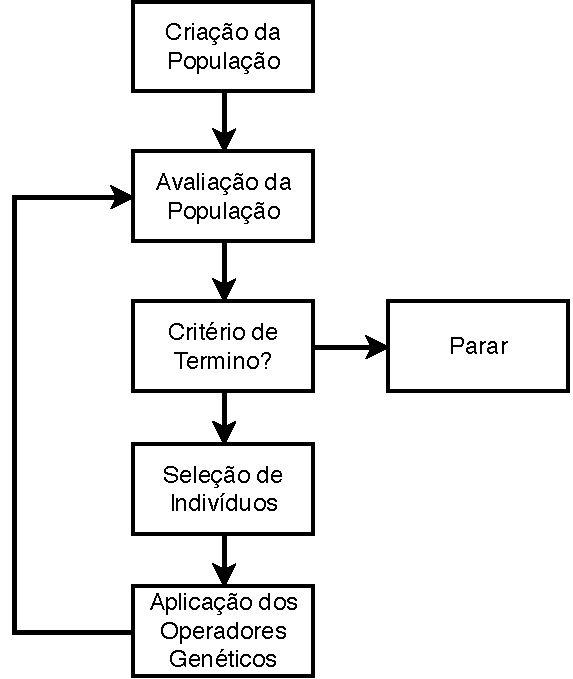
\includegraphics[width=0.4\linewidth]{02_desenvolvimento/01_Pg_Fig_ExCicloSimples}
\caption{Aprendizagem evolucionária.}\label{fig:1pg-ciclosimples}
\end{figure}

O primeiro passo é a criação da população de indivíduos, de acordo com a representação escolhida. A abordagem deste trabalho utiliza o conceito proposto por Koza~\cite{koza92bookGp}, onde cada indivíduo possui uma estrutura recursiva (semelhante a uma árvore) que representa, em sua essência, um programa de computador.

Para os problemas que serão abordados, em suma, o objetivo é encontrar uma lei de controle capaz de estabilizar o sistema ou alcançar um propósito definido. Por exemplo, um indivíduo aleatório inicializado poderia ter uma estrutura igual à apresentada na Figura \ref{fig:1pg-exrepresentacao}. A lei de controle seria dada pela expressão matemática que resulta do cálculo recursivo da árvore que representa o indivíduo.

\begin{figure}[!htb]
\centering
\includegraphics[width=0.4\linewidth]{02_desenvolvimento/01_Pg_Fig_ExRepresentacao.png}
\caption{Um indivíduo aleatório representando uma lei de controle. $c_1$ e $c_2$ são constantes. $s_1$ e $s_2$ são leituras de um sensor.}\label{fig:1pg-exrepresentacao}
\end{figure}

Na Figura \ref{fig:1pg-exrepresentacao}, círculos representam \textbf{operadores}, enquanto os quadrados, \textbf{variáveis terminais}. Como a representação utilizada se assemelha à uma árvore, é possível definir como:

\begin{itemize}[label=\raisebox{0.25ex}{\tiny$\bullet$}]
	\item \underline{Raiz:} o operador do topo (i.e., que não é argumento de outro operador).
	\item \underline{Ramo:} a estrutura composta por um operador e seus argumentos (mesmo que estes sejam outros ramos).
	\item \underline{Folha:} a variável terminal, isto é, uma constante ou uma variável. Caracteriza-se por não ser operador e, portanto, não possui argumentos.
\end{itemize}

Os operadores podem ser matemáticos ou lógicos. Quanto à aridade, pode-se utilizar operadores que aceitem um ou mais argumentos. As variáveis terminais podem ser constantes como $1$ e $0$ ou até números aleatórios dentro de uma faixa. Em problemas de controle é comum admitir como variáveis terminais uma leitura de sensor, por exemplo.

Em linguagens de programação baseadas no processamento de listas, o indivíduo da Figura \ref{fig:1pg-exrepresentacao} poderia ser descrito através da expressão:

\begin{equation*}
(+(*(s_1)(c_1))(-(s_1)(\cos(c_2))))
\end{equation*}

Geralmente, a representação em forma de árvore é mais intuitiva. Entretanto, costuma ser mais eficiente trabalhar com sequências de caracteres, representando uma lista.

É possível estipular, também, um tamanho mínimo e máximo de cada árvore, eliminando assim expressões muito simples, em que sabemos não servir como solução para o problema, ou soluções demasiadamente complexas.

Existem diversas variações da estrutura em forma de árvore. Na programação genética cartesiana~\cite{miller08Cgp}, por exemplo, cada variável de entrada pode servir de operando para mais de um operador. Na programação genética linear~\cite{douglas05Pgl}, um indivíduo é um programa de computador com instruções independentes, executadas de forma sequencial.

A inicialização de cada indivíduo é feita de forma aleatória, respeitando um dado conjunto de operadores $\mathcal{O}$, variáveis terminais $\mathcal{V}$ e nível (ou número de camadas) $\mathcal{D} \in (D_{min}, D_{max})$.

Por exemplo, se definirmos:

\begin{align}
\label{eq:1pg-caractexpopinicial}
\mathcal{O} &= \{+, -, *\} \nonumber\\
\mathcal{V} &= \{1, 0, 3\}\\
\mathcal{D} &= \{1, 2\} \nonumber
\end{align}

Indivíduos como os da Figura \ref{fig:1pg-expopinicial} seriam possíveis elementos dessa população.

\begin{figure}[!htb]
\centering
\includegraphics[width=0.8\linewidth]{02_desenvolvimento/01_Pg_Fig_ExInicializacao.png}
\caption{Um exemplo de inicialização de uma população de três indivíduos, com as características descritas na Equação \ref{eq:1pg-caractexpopinicial}.}\label{fig:1pg-expopinicial}
\end{figure}

Após a inicialização da população é feita a avaliação de cada indivíduo. O objetivo desta etapa é verificar a aptidão de todos os membros da população, através de uma medida que reflita o que se busca como solução para o problema, ou seja, a função que determina o desempenho da solução é específica a cada aplicação.

Em problemas de controle, geralmente o objetivo é manter a posição de um objeto o mais próximo possível de um valor de referência, $X_{ref}$, utilizando uma medição do valor atual, $X_{med}$. Diagramas como o da Figura \ref{fig:1pg-malhacontroleclassico} são comuns na teoria clássica de controle.

\begin{figure}[H]
	\centering
	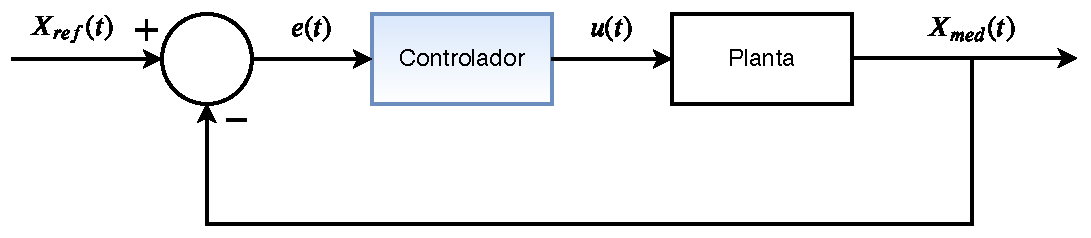
\includegraphics[width=0.85\linewidth]{02_desenvolvimento/01_Pg_Fig_MalhaControleClassico.pdf}
	\caption{Sistema de controle por realimentação. O sinal de erro, $\bm{e(t)}$, é a entrada do controlador, que atua na planta através do sinal de controle, $\bm{u(t)}$.}
	\label{fig:1pg-malhacontroleclassico}
\end{figure}

A avaliação de um indivíduo pode ser representada como uma função custo, $\mathbf{J}$. O objetivo do algoritmo é, portanto, achar um sinal de controle que minimiza $\mathbf{J}$, uma métrica que leva em consideração o erro $e(t)$, em um intervalo de tempo.

% Uma função custo é implementada de modo que penalize desvios de um estado de referência, conforme indica a Equação \ref{eq:1pg-funcaoCusto}.

\begin{equation}\label{eq:1pg-funcaoCusto}
J = \dfrac{1}{T}\int_0^{T}j(e(t))\,dt = \dfrac{1}{T}\int_0^T\left(X_{ref}-X_{med}\right)^2\,dt
\end{equation}

Na programação genética, o indivíduo age como o controlador da Figura \ref{fig:1pg-malhacontroleclassico}, porém, recebe apenas uma medida do estado atual para guiar sua atuação. Isto é, o erro é utilizado apenas por um processo externo à interação do indivíduo com a planta, como um meio de realizar o cálculo de $\mathbf{J}$. Este, por sua vez, é um valor que pode representar a aptidão deste indivíduo. Este processo pode ser observado na Figura \ref{fig:1pg-malhacontrolepg}.

\begin{figure}[H]
	\centering
	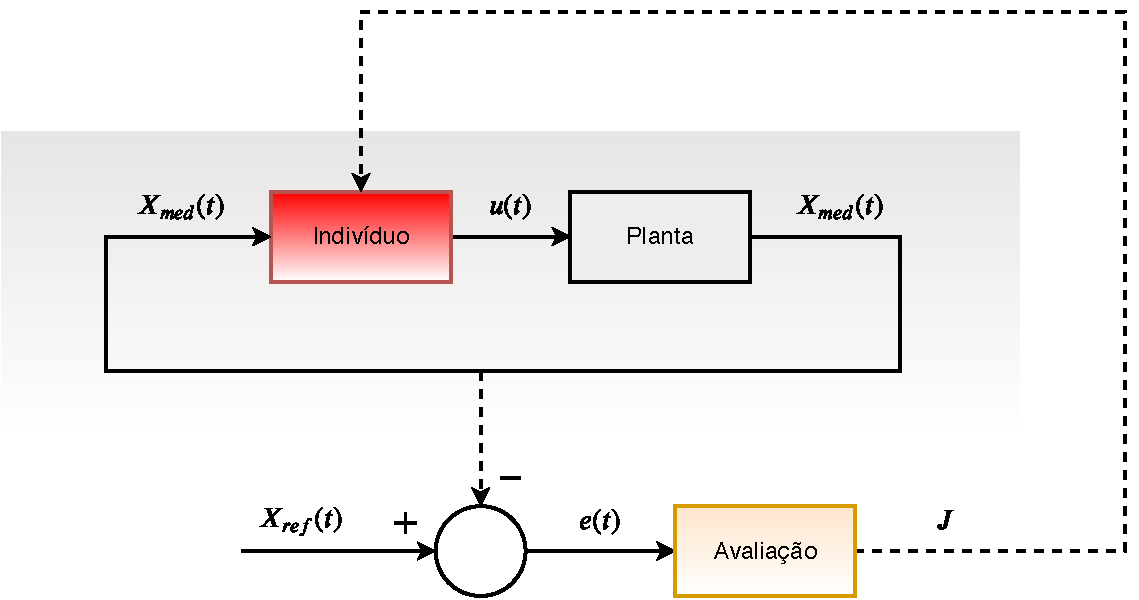
\includegraphics[width=0.85\linewidth]{02_desenvolvimento/01_Pg_Fig_MalhaControlePG.pdf}
	\caption{O indivíduo interage com a planta utilizando apenas medições do estado atual do sistema.}
	\label{fig:1pg-malhacontrolepg}
\end{figure}

Com uma medida de aptidão associada a cada indivíduo, é possível selecionar os mais aptos. Um método básico e eficaz de seleção é comparar dois indivíduos aleatórios na população, utilizando a métrica de desempenho estipulada, e escolher o que possui maior valor numérico de aptidão.

Esse método conhecido como \textit{torneio} pode ser feito em dois ou mais níveis, isto é, são escolhidos quatro ou mais indivíduos aleatórios na população, realizando comparações dois a dois, de modo que apenas um indivíduo seja escolhido ao final.

Um dos operadores genéticos é aplicado neste indivíduo e a solução gerada é inserida em uma nova população. O processo de seleção, aplicação de operadores genéticos e eventual inserção do indivíduo se repete até que o número de indivíduos gerados seja igual a quantidade de membros da população antiga.

Para cada indivíduo selecionado, apenas uma operação genética é aplicada, após ser escolhida de forma aleatória. Cada operação genética tem, portanto, uma probabilidade de ser selecionada. A soma das probabilidades de cada operação deve ser igual a um.

%\begin{itemize}[label=\raisebox{0.25ex}{\tiny$\bullet$}]
% \item $P_c$: probabilidade de cruzamento.
% \item $P_m$: probabilidade de mutação.
% \item $P_r$: probabilidade de replicação.
%\end{itemize}

\begin{equation}
\left.\begin{aligned}
P_c&\text{: probabilidade de cruzamento} \\
P_m&\text{: probabilidade de mutação} \\
P_r&\text{: probabilidade de replicação}
\end{aligned}\right\} P_c+P_m+P_r=1
\end{equation}

É interessante lembrar que o ciclo evolutivo é uma \textbf{busca} por soluções. Nesse contexto, são comuns na literatura os termos \textbf{exploration} e \textbf{exploitation}, que se referem a exploração, entretanto \textit{exploration} se refere a uma busca em larga escala, enquanto \textit{exploitation} refere-se a uma procura local.

De acordo com Brunton et al. \cite{duriez17bookMlc}, a procura pelo mínimo da função custo pode ser representada por gráficos semelhantes ao da Figura \ref{fig:1pg-grafbuscaexpl}, onde a operação de cruzamento realiza uma busca local (exploitation), enquanto a mutação opera em larga escala (exploration).


\begin{figure}[!!htb]
\centering
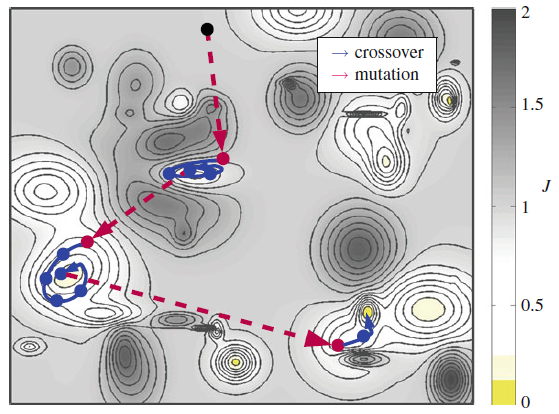
\includegraphics[width=0.7\linewidth]{02_desenvolvimento/01_Pg_Fig_GraficoBuscaExploration.png}
\captionsource{Representação 2D da busca pelo mínimo da função custo. A operação de mutação permite uma busca em larga escala (em vermelho). Em azul, a operação de cruzamento busca a convergência para o mínimo local.}{\cite{duriez17bookMlc}}\label{fig:1pg-grafbuscaexpl}
\end{figure}

A operação de cruzamento, demonstrada na Figura \ref{fig:1pg-excruzamento}, é realizada em dois indivíduos selecionados, isto é, aptos de acordo com o critério de desempenho escolhido. É razoável, portanto, que seja responsável pela convergência local, pois os novos indivíduos gerados possuem \textbf{toda} sua estrutura formada por ramos de soluções consideradas boas. Já no caso da mutação, o novo indivíduo possuirá uma parcela de sua estrutura sendo gerada de forma aleatória, o que não garante convergência, porém é útil para explorar o espaço de possíveis soluções.

A operação genética de \textit{mutação} começa ao selecionar um ponto aleatório na árvore, podendo este ser interno ou externo (operadores ou variáveis terminais). A mutação remove este ramo (ou folha) e uma nova sub-árvore é gerada aleatoriamente, produzindo uma variável terminal (Figura \ref{fig:1pg-exmutvarterm}) ou um ramo (Figura \ref{fig:1pg-exmutramo}).

\begin{figure}[H]
\centering
\includegraphics[width=1\linewidth]{02_desenvolvimento/01_Pg_Fig_ExMutacaoVarTerm.png}
\caption{Mutação aplicada à um ponto correspondente a uma variável terminal gerando um \textit{ramo}.}\label{fig:1pg-exmutvarterm}
\end{figure}

\begin{figure}[H]
\centering
\includegraphics[width=0.9\linewidth]{02_desenvolvimento/01_Pg_Fig_ExMutacaoRamo.png}
\caption{Mutação aplicada em um ponto correspondente a um \textit{ramo}. A nova sub-árvore possui apenas uma \textit{variável terminal}.}\label{fig:1pg-exmutramo}
\end{figure}

A operação de \textit{cruzamento} atua a partir de dois indivíduos selecionados. Assim como na operação de \textit{mutação}, um ponto aleatório na árvore de cada indivíduo é escolhido aleatoriamente e os ramos correspondentes são trocados entre as soluções (Figura \ref{fig:1pg-excruzamento}).

\begin{figure}[H]
\centering
\includegraphics[width=0.8\linewidth]{02_desenvolvimento/01_Pg_Fig_ExCruzamento.png}
\caption{Exemplo da operação de cruzamento atuando em dois indivíduos.}\label{fig:1pg-excruzamento}
\end{figure}

A \textit{replicação} é um operador genético simples em que um indivíduo selecionado é copiado diretamente para a próxima geração, sem qualquer alteração em sua estrutura, conforme indica a Figura \ref{fig:1pg-exreplicacao}.

\begin{figure}[H]
\centering
\includegraphics[width=0.9\linewidth]{02_desenvolvimento/01_Pg_Fig_ExReplicacao.png}
\caption{Operação de \textit{replicação} aplicada em um indivíduo selecionado.}\label{fig:1pg-exreplicacao}
\end{figure}

Koza~\cite{koza92bookGp} menciona outras operações genéticas como a \textit{edição}, cuja função é editar e simplificar as expressões das árvores; \textit{Permutação}, uma generalização do operador de inversão aplicado em algoritmos genéticos de representações fixas; \textit{Encapsulamento}, um método de identificação de ramos úteis que podem ser referenciados e \textit{elitismo}, que copia os indivíduos de maior aptidão diretamente para a próxima geração.

Geralmente, o critério de término do ciclo evolutivo é um número limite de gerações. Alguns problemas permitem a criação de um critério de desempenho, isto é, o ciclo evolutivo se repete até que um indivíduo obtenha um determinado valor de aptidão.

Uma implementação de programação genética não se torna completa sem o estabelecimento de alguns parâmetros de controle, como por exemplo, o número de indivíduos da população ou a probabilidade de cada operação genética. Os principais parâmetros da PG são enumerados a seguir:

\begin{enumerate}
\item \textbf{Em relação à população:}
\begin{enumerate}[label={\alph*)}]
\item Número de indivíduos da população: $M$
\item Número máximo de gerações: $G$
\item Método de inicialização
\item Método de seleção de indivíduos
\end{enumerate}
\item \textbf{Em relação à representação do indivíduo:}
\begin{enumerate}[label={\alph*)}]
\item Conjunto de operações em ramos: $\mathcal{O}$
\item Conjunto de variáveis terminais: $\mathcal{V}$
\item Mínima profundidade inicial da árvore: $D_{min}$
\item Máxima profundidade inicial da árvore: $D_{max}$
\end{enumerate}
\item \textbf{Em relação às operações genéticas:}
\begin{enumerate}[label={\alph*)}]
\item Probabilidade de cruzamento: $P_c$
\item Probabilidade de mutação: $P_m$
\item Probabilidade de replicação: $P_r$
\end{enumerate}
\end{enumerate}

A partir dos parâmetros estabelecidos e dos métodos esclarecidos neste capítulo, é possível reformular o ciclo da Figura \ref{fig:1pg-ciclosimples} para a inclusão de outros detalhes.

\begin{figure}[!h]
\centering
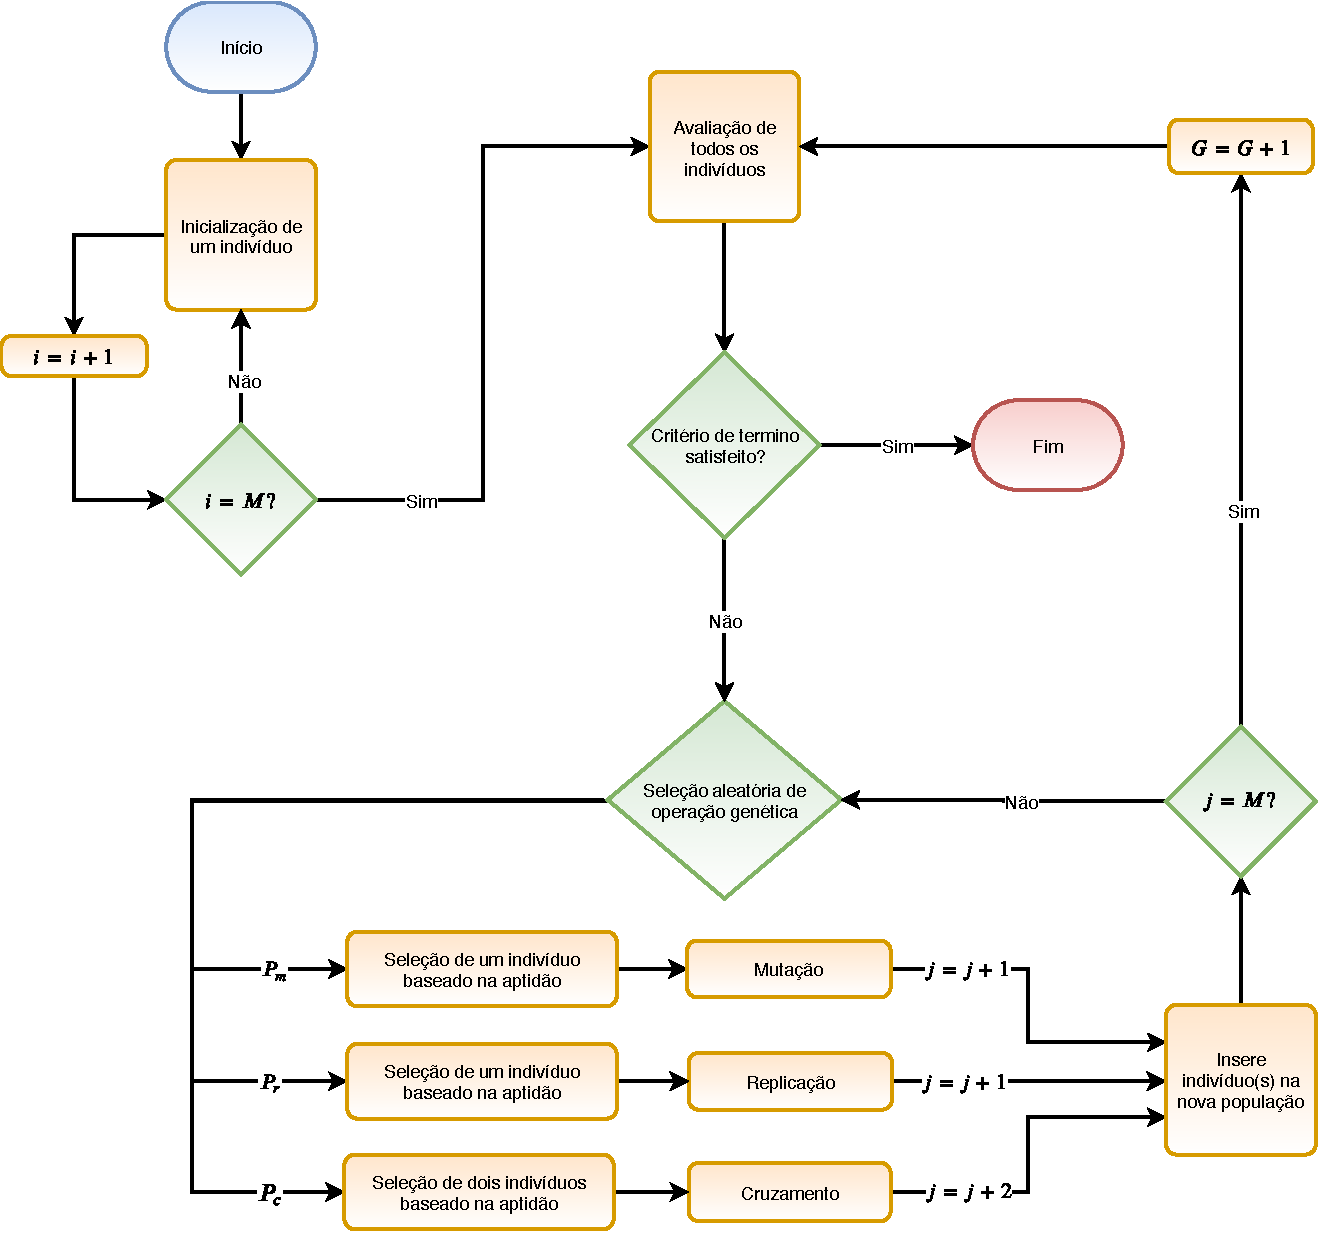
\includegraphics[width=1\linewidth]{02_desenvolvimento/01_Pg_Fig_CicloCompleto.pdf}
\caption{Ciclo evolucionário para programação genética.}\label{fig:1pg-ciclocompleto}
\end{figure}

Com base no fluxograma da Figura \ref{fig:1pg-ciclocompleto} é possível realizar a programação genética para um problema genérico. Resta, portanto, verificar as particularidades da implementação para cada problema abordado.


